\chapter{Introduction}
\label{chp:introduction}

% printer: Tethered flight control of a small quadrotor robot for stippling \cite{galea_iros_2017}

%Example of energy harvesting: Prolonged energy harvesting for ingestible devices~\cite{plonski_tranro_2016}
%Drug delivery

% Estabish your territory

Miniature robots with limited capabilities can work together as a collective to achieve more than an individual could by itself, but are still far from being applicable in real world applications~\cite{barca_sekercioglu_2013}.
The future potential of collectives of small robots, i.e. swarms, is widely recognized to have applications in surveillance, search and rescue, and exploration.
Swarms have been proposed as a new form of user interface, robots can display information and interact with users on tabletops~\cite{legoc_uist_2016}, unmodified clothing~\cite{dementyev_uist_2016} and can be an educational toy for kids~\cite{sony_toio_2017}, as seen in Figure \ref{fig:int_example_sui}.
%\hfill \break

% Establish nice
% Motivation for this work: Why do we want to remove the battery?

However, one of the fundamental issues that needs to be addressed before swarm robotics can advance is related to energy.
Small lithium batteries are currently powering the robots and limit their operation time to only a few hours. 
The energy density of batteries has improved less than one order of magnitude since 1945, while in comparison the energy efficiency of computing has improved 12 orders of magnitude~\cite{patel_pvc_2017}.
The last major advancement in battery technology is 25 years old and came with the introduction of Li-ion batteries.
Additionally, any new big improvements in energy density of batteries is not likely to happen anytime soon, as new battery technologies are often overhyped and slow to emerge~\cite{zachary_spec_2016}.
%	\hfill \break

%TODO introduce current research

% Propose a solution: Energy harvesting
% And discuss current solutions to autonomus operation / battery replenishment

Stable energy supplies are required to allow long term persistent operation of robots.
Wireless sensor nodes that rely on energy harvesting have already been emerging, are highly energy constrained but fully eliminate the need for batteries~\cite{wisp5_wiki_2017}.
In contrary, different replenishment methods for robot batteries are currently used, robots can be moved to a charging station leaving them nonoperational, and manual recharging or battery replacement results in a high strain on maintenance.
Therefore, relaxing the stable energy supply constraint by allowing a transient supply of harvested energy could be a potent area of research.

% 4 lines left!
\newpage

\begin{figure}
	\begin{subfigure}[b]{0.32\textwidth}
		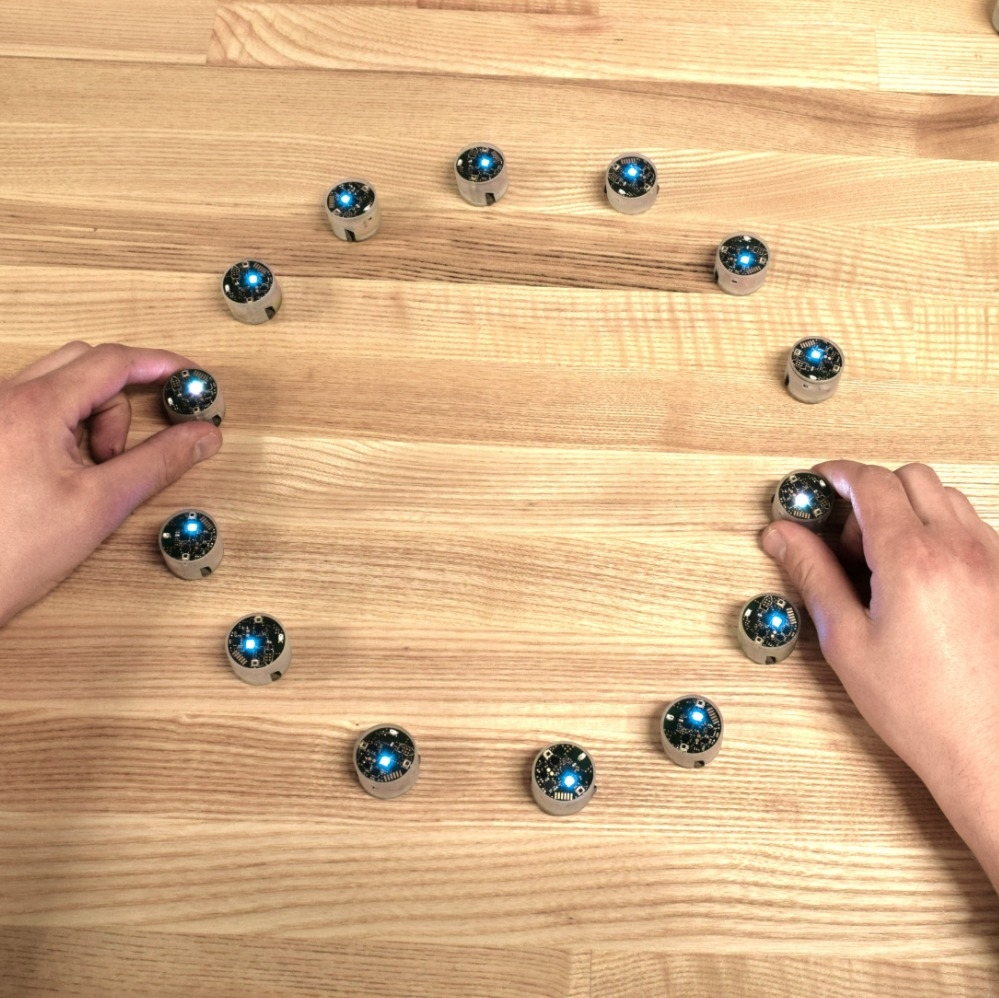
\includegraphics[width=\textwidth]{pics/zooids.jpg}
		\caption{Zooids}
		\label{fig:int_zooids}
	\end{subfigure}
	\begin{subfigure}[b]{0.324\textwidth}
		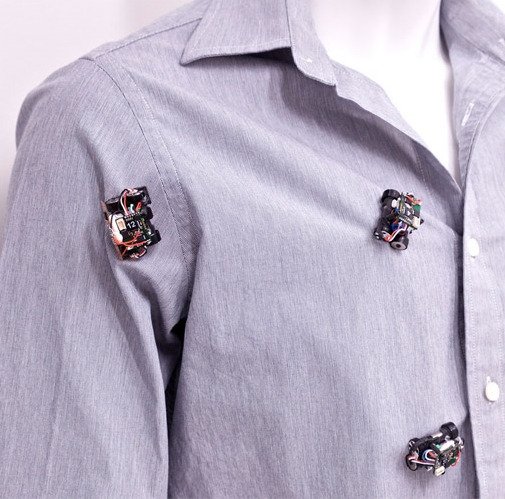
\includegraphics[width=\textwidth]{pics/rovables.jpg}
		\caption{Rovables}
		\label{fig:int_roverables}
	\end{subfigure}
	\begin{subfigure}[b]{0.323\textwidth}
		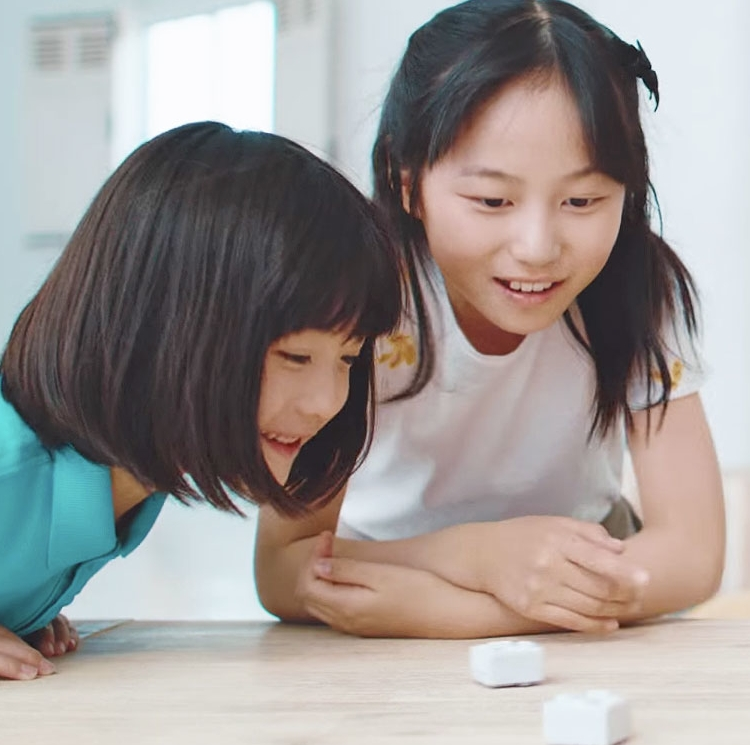
\includegraphics[width=\textwidth]{pics/toio.jpg}
		\caption{Sony Toio}
		\label{fig:int_toio}
	\end{subfigure}
	\caption{Current applications for small robotic platforms.}
	\label{fig:int_example_sui}
\end{figure}

\section{Problem statement}

% What why how

% Intermittently powered robots, that purely rely on harvested power are currently non existent.

% swarm robots ie kilobot operate form batteries -> need recharging -> move to tosti irond cannot be used while charging .

Replacing a battery with an energy harvesting system could make a robot self sufficient and energy-autonomous. 
This however introduces a new phenomenon to take into account; the intermittent availability of energy produces frequent power interrupts.
The possibility of sudden power loss is currently not considered when developing control software for a robot, and for this reason can not be used without adaption.
%\hfill \break

Secondly, applicable sensors and/or sensing frequency may be constrained due to the limited energy budget.
The largest part of the energy budget will already be consumed by the actuators that supply movement to the robot.
Not every locomotion type currently used may reliable and/or accurate under the frequent power interruption.
Therefore the research question this work addresses is:

\begin{center}
	\textit{What is the effect of intermittentcy on the movement accuracy of a transiently powered robot without external feedback?}
	%\textit{How to enable a transiently powered robot to operate autonomously?}
\end{center}

\section{Contributions}
Current robots assume that a task can only be completed if sufficient energy is left in the batteries, which inherently limits their operation time. 
This research will explore the feasibility of a miniature battery-free robot, allowing persistent operation while being supplied by a small and intermittent source of energy.
%This is the first study of transiently powered robots, unaware of any platforms being implemented and are operating under the constant threat of power loss. 
The list of contributions is as follows:

\begin{enumerate}

%\item A simple model is developed showing the relation between the energy stored, weight of the robot, frequency of power cycles and distance covered with a single charge.

\item Design of a battery-free robot that purely operates from harvested energy, with basic capabilities allowing autonomous operation.

%TODO state results of implementation in contribution
\item Implementation of a control algorithm, that allows the robot to finish a movement across power cycles.

%\item Evaluation of the battery-free robot compared to a battery powered robot in terms of, weight, speed and accuracy of movement.


\end{enumerate}


\section{Thesis Outline}

The rest of the this is organized as follows: Chapter \ref{chp:related_work} provides background information and related work.
The preliminaries in designing the transiently-powered robot are presented in Chapter \ref{chp:preliminaries}.
In Chapter \ref{chp:design_and_implementation} explains the hardware design and software implementation..
Next, the performance of the transiently powered robot will be evaluated in Chapter \ref{chp:evaluation}.
Finally, Chapter \ref{chp:summary} concludes this thesis and proposes potential future work.



